% Source: https://texample.net/tikz/examples/pera-model/

% The Purdue Enterprise Reference Architecture (PERA) model.
% Author: Erno Pentzin (2013)
\documentclass{article}
\usepackage{tikz}
\usetikzlibrary{chains}
\begin{document}

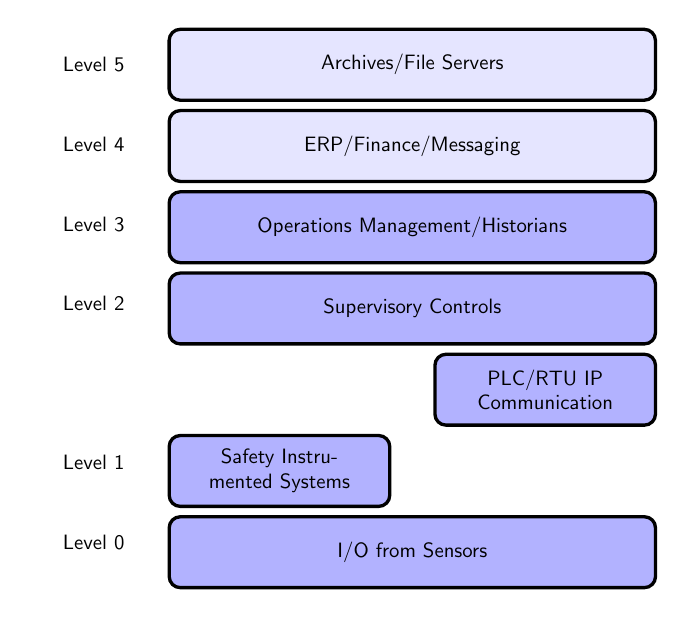
\begin{tikzpicture}[
    scale=0.75,
    start chain=1 going below,
    start chain=2 going right,
    node distance=1mm,
    desc/.style={
        scale=0.75,
        on chain=2,
        rectangle,
        rounded corners,
        draw=black,
        very thick,
        text centered,
        text width=8cm,
        minimum height=12mm,
        fill=blue!30
        },
    it/.style={
        fill=blue!10
    },
    level/.style={
        scale=0.75,
        on chain=1,
        minimum height=12mm,
        text width=2cm,
        text centered
    },
    every node/.style={font=\sffamily}
]

% Levels
\node [level] (Level 5) {Level 5};
\node [level] (Level 4) {Level 4};
\node [level] (Level 3) {Level 3};
\node [level] (Level 2) {Level 2};
\node [level] (Level 1.5) { };
\node [level] (Level 1) {Level 1};
\node [level] (Level 0) {Level 0};

% Descriptions
\chainin (Level 5); % Start right of Level 5
% IT levels
\node [desc, it] (Archives) {Archives/File Servers};
\node [desc, it, continue chain=going below] (ERP) {ERP/Finance/Messaging};
% ICS levels
\node [desc] (Operations) {Operations Management/Historians};
\node [desc] (Supervisory) {Supervisory Controls};
\node [desc, text width=3.5cm, xshift=2.25cm] (PLC) {PLC/RTU IP Communication};
\node [desc, text width=3.5cm, xshift=-4.5cm] (SIS) {Safety Instrumented Systems};
\node [desc, xshift=2.25cm] (IO) {I/O from Sensors};

\end{tikzpicture}

\end{document}
